A torus can not have a hyperbolic structure, it has naturally a flat structure as the quotient $\mathbb{R}^2 / \mathbb{Z}^2$.
This changes when one study the one ponctured torus. It is a torus $S$ where we choose a point $p$ and remove it (or just marked it).

The construction of this object can be done in two manier at least.
For the first construction, one have to choose a hyperbolic octogone where one side have length $0$ and the two other one $l$, then we sew the border of two of this octogone which give a pair of pant. Finally we can glued with a twist $\tau$ to have the one ponctured torus.

A second construction is given by the representation. Given two hyperbolic isomorphism of $\mathbb{H}$ $A$ and $B$ with different fixed point on $\delta \mathbb{H}$ and with $H := ABA^{-1}B^{-1}$ the commutator should be a parabolic element.

A fundamental domaine is given by the following image:


%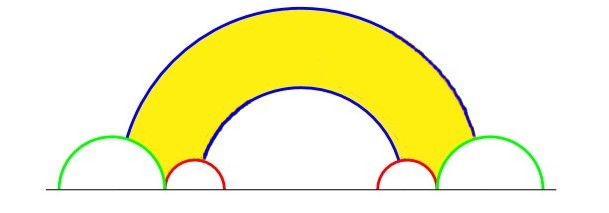
\includegraphics{Image/OnceTorusFundamentalDomaine.jpg}


\begin{figure}[h]
\centering
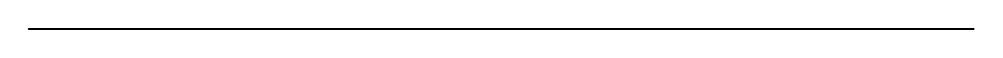
\begin{tikzpicture}[scale=1,cap=round]
\tkzInit[xmin=-4, xmax=4, ymin=0, ymax=3]
\tkzClip
%Draw circle
\tkzDefPoint(0,0){O} %define origin
\tkzDefPoint(-2,0){x1}
\tkzDefPoint(2,0){x2}
\tkzDefPoint(-3,0){y1}
\tkzDefPoint(3,0){y2}
\tkzDefPoint(-2.25,0){c1}
\tkzDefPoint(2.25,0){c2}

\tkzDrawCircle[thick, fill=gray!30](O,y1){circleOy}
\tkzDrawCircle[thick, fill=white](O,x1){circleOx}

\tkzDrawCircle[thick, fill=white](x1,c1){circlex1}
\tkzDrawCircle[thick, fill=white](x2,c2){circlex2}
\tkzDrawCircle[thick, fill=white](y1,c1){circley1}
\tkzDrawCircle[thick, fill=white](y2,c2){circley2}

\draw[thick] (-6, 0) -- (6, 0); %horizontal line

\end{tikzpicture}
\caption{A fundamental domain of a punctured torus}
\end{figure}


Given two generators $\alpha$ and $\beta$ of $\pi_1(S)$, two closed curves non homotopically trivial which intersect one, one can parametrize all other lamination.
Indeed a given lamination $\lambda \in \mathcal{ML}$ is determined by the couple $(i(\alpha,\lambda),i(\beta,\lambda))$ where $i(.,.)$ is the geometric intersection number.

We have this useful lemma to estimate the length of the systole function in the Teichmuller space.

\begin{lem}
Pick $\gamma$ a simple closed geodesic, and $X \in \mathcal{T}(S_{1,1)}$, if $X$ has Fenchel-Nielsen coordinate $(L,\frac{p}{q})$ with respect to $\gamma$, where $gcd(p,q)=1$ and $\frac{p}{q} \in ]0;1[$, then \[
C_1(L) e^{\frac{-L}{2q}} < l_{sys}(X) < C_2(L) e^{\frac{-L}{2q}}
\]
where $C_1(L)$, $C_2(L)$ both limits to $4$ when $p$, $q$ are fixed and $L$ goes to $\infty$
\end{lem}

\begin{proof}
Let $R(L)$ be the length of the shortest geodesic arc with endpoints on $\gamma$. We have \[
R(L)= 2 log(coth(L/4))=2 log(\frac{e^{l/2}+1}{e^{l/2}-1})
\]
By the collar lemma \ref{ColLem}.
Then if we take $\alpha$ a simple closed curve that intersect $\gamma$, $q$ times exactly, we obtain the following inequality with $a=l_\alpha(X)$ \[
q R(a) < L < q R(a) + \frac{qa}{2}
\]
Reorganizing the termes we have \[
e^{-a/4}tanh(a/4) < e^{-L/2q} < tanh(a/4)
\]
As $a \rightarrow 0$ then $L \rightarrow \infty$
\[
C_1(L) e^{\frac{-L}{2q}} < a < C_2(L) e^{\frac{-L}{2q}}
\]
To complete the proof , we need to show that the length of $\alpha$ is shorter than any other géodesic closed curves, but with the collar lemma there is only one systole whose length goes to $0$ and this is the case for $\alpha$ as $L \rightarrow \infty$.
%TODO detailler la preuve

If we don't don any approximation we have \[
2 ln(\frac{1+e^{-L/2q}}{1-e^{-L/2q}}) < a
\]

\end{proof}

\begin{thm} Let $\nu(S_{1,1})$ be the finite measure on $\mathcal{P}^1 \mathcal{M}(S_{1,1})$. Then \[
\nu(S_{1,1})\{ (X,\lambda) \in \mathcal{P}^1 \mathcal{M}(S_{1,1}) | l_{sys}(X,\lambda) < \epsilon \} = O(\frac{\epsilon}{log \epsilon})
\] as $\epsilon \rightarrow 0 $
\end{thm}

%Portion de preuve
\hrulefill

Let fix $\epsilon=l_{sys}(X)$, and $T > 0 $, then $\exists N=N(\epsilon,T)$ such that $\forall n \geq N$ \[
| l_{sys}E_t(X,\lambda)-l_{sys}E_t(X,\frac{\gamma_n}{l_{\gamma_n}(X)})| < \epsilon
\]

So we calculate $T_n$ such that $\forall |t| < T_n$,
 $l_{sys}E_t(X,\frac{\gamma_n}{l_{\gamma_n}(X)}) < 2 \epsilon$
and $T=liminf T_n$. If $T>0$, $\exists N_1$ such that $\forall n \geq N_1$, $T_n \geq \frac{T}{2}$.

Then we set $N_2=N(\epsilon,T/2)$ and we have $l_{sys}E_t(x,\lambda) \leq 2.5 \epsilon $, $\forall 0 \leq t \leq T/2$


\hrulefill

We have two useful tools to understand the length fonction along a earthquake path.

\begin{lem}
Let $X \in \mathcal{T}(S_g)$, and $\gamma$ a curve which is part of a pant decomposition.
 $\chi_s$
  is the twist of length $s$ around $\gamma$, and $b$ a closed curve with $i(b,\gamma) > 0$ then $s \mapsto l_{\chi_s}(b)$ is strictly convex.
\end{lem}
\cite{farb2011primer} proposition 10.8

\begin{lem}
If $\alpha$ is a closed curve, $\gamma$ an other closed curve and $\lambda$ a lamination.\[
\begin{array}{crcl}

\frac{dl_{\alpha}}{dt}(0) & = & \sum_{p_i \in \alpha \cap \gamma} cos(\theta_{p_i}) \\

\frac{dl_{\alpha}}{dt}(0) & = & \int_{ \alpha} cos(\theta) d \theta

\end{array}
\]
\end{lem}
\cite{NielsenRealizationPro} Corollary 3.3 and 3.4
